\documentclass{article}
\usepackage[utf8x]{inputenc}
\usepackage[T1, T2A]{fontenc}
\usepackage[russian]{babel}
\usepackage{amsmath}
\usepackage{graphicx} 
\usepackage{amssymb}
\setlength\parindent{0pt}
\usepackage[parfill]{parskip}
\pagenumbering{gobble}

\begin{document}
Будем следить за положением центра окружности. Ясно, что можно ограничить рассмотрение внутренностью одного прямоугольника. Нетрудно видеть, что для того, чтобы окружность пересекала ровно три прямоугольника, должны выполняться два условия:\\
(1) расстояния от центра до двух ближайших сторон прямоугольника должны быть меньше $4$;\\
(2) расстояние до ближайшей вершины прямоугольника должно быть больше $4$.\\
Зная это, мы можем изобразить множество точек, удовлетворяющих этим условиям:
\begin{figure}[!h]
\center{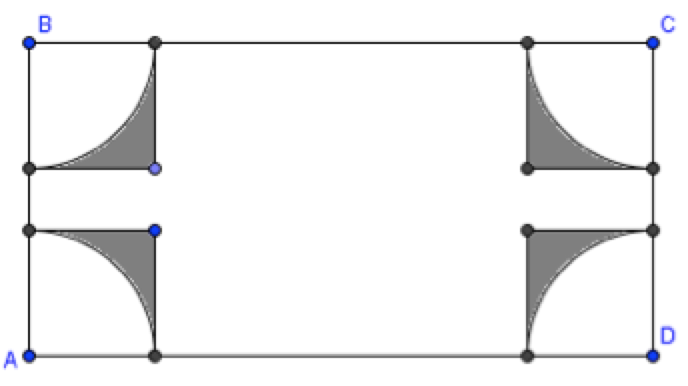
\includegraphics[width=0.6\textwidth]{rectangle}}
\end{figure}
\\Следовательно, искомая вероятность равна
$$\frac{S_{\text{закрашенной части}}}{S_{\text{прямоугольника}}} = \frac{4 \cdot (16 - \frac14 \cdot 16\pi)}{10 \cdot 20} = \frac{16 - 4\pi}{50} = \frac{8 - 2\pi}{25}.$$
\end{document}
